\section{Experiments}\label{sec:experiments}

Every experiment of this section fixes its measured quantity before the runs, compares each arm with controls that spend the same kind of budget, and counts a step only after the check that the run itself performs. The unit of cost is one check of one closed composite. The experiments are, in order: a router of strategies on the two Millennium benchmarks; the crossing network on Erd\H{o}s problem 1183, where the only advance came from a change of representation; the crossing network on Yang--Mills and Hodge, where it reaches the range $\beta_{W}<\frac13$; the booster layer; the memory, the channel and the agents; and the barrier and pattern matrix.

\subsection{A router of strategies on Hodge and Yang--Mills}\label{ssec:router}

In its first form the package represented each of the two open problems as a tree whose root is the statement and whose leaves are the pieces it splits into: a faithful Lean statement, the lattice gap at strong coupling, fine-scale control at weak coupling, the crossover window at order-one coupling with two attempts on it, and the continuum limit for Yang--Mills; a faithful Lean statement, (F2) in dimension at most five, for CM abelian varieties, for split Weil eightfolds and through a semiregular object on $E_{0}^{6}$, and (F3$'$) for the square of a K3 surface with real multiplication and for Fermat fourfolds for Hodge. A run picks a leaf and one of eight moves (reduction, special case and lift, certificate, construction, counterexample, flow with surgery, descent, physics first), and a move is accepted only when a computation of the package checks it. These are the trees of six and eight leaves on which the router was run; Section~\ref{ssec:headline} adds the leaves the crossing network opened. Five policies choose the move: uniformly; by the prior of the Lean-formalised manuscripts of \cite{OAI26b}; by a router that averages that prior with the share of the settled Erd\H{o}s problems solved by each move and is reinforced by accepted steps; by the profile of a local language model, the softmax of the next-token logits of a model with $1.5\times10^{9}$ parameters over the letters of the eight moves \cite{Qwe24}; and by the mixture of the last two with weight $\frac12$.

Over $200$ seeds of $12$ rounds every policy finds the same two accepted steps, the reduction of the Hodge conjecture for a Fermat fourfold of degree $m$ to the degrees with leftover characters, by Shioda's criterion for zero-sum pairs and triples, and the strong-coupling gap $m\ge-\log(9\beta_{W}/2)$ for $\beta_{W}<\frac29$. The mean number of attempts before both are found is $36.3$ for the uniform policy, $38.3$ for the corpus prior, $35.4$ for the router, $26.3$ for the profile of the model and $33.5$ for the mixture; of $65$ to $67$ attempts per run, between $50.9$ and $52.9$ go to moves that have no checkable formulation at their leaf. The model's profile is the best of the five, by a factor of $1.38$ over the uniform policy, and no policy moves any open leaf. Both accepted steps are results of \cite{BB26c,BB26d}; the benchmark measures how fast a policy finds a step that a computation can check, and on these trees the only such steps are known ones. Moving a leaf needed a different proposer, one that combines known constructions instead of choosing among moves, and that is the crossing network of the next subsection.


\subsection{A chain reaction of constructions}\label{ssec:crossing}

The library of the package records known constructions with their provenance. The crossing network makes each of them a typed node and breeds new constructions from pairs of old ones, keeping an offspring only if it passes a check, so that every survivor is a checked construction that may seed the next generation. The experiment asks whether learning which crosses survive produces more new constructions than crossing at random.

\emph{The domain.} Let $f(n)$ be the largest $N$ such that every $2$-colouring of the subsets of $[n]=\{1,\dots,n\}$ has a monochromatic family of $N$ sets closed under union and intersection, Erd\H{o}s problem 1183 \cite{Blo1183}. A maximal chain has $n+1$ members and each of its colour classes is closed under both operations, so $f(n)\ge\lceil(n+1)/2\rceil$, and Chojecki proved $f(n)\le(3+o(1))\,n\log_{2}n$ \cite{Cho26}.\footnote{D.~Bhattacharjee, P.~Mandal and U.~Bhattacharya, \emph{Resolving Erd\H{o}s--Ulam monochromatic union-closed family conjectures}, arXiv:2610.02833v1 (2 October 2026), doi:10.48550/arXiv.2610.02833, with Lean~4 archive doi:10.5281/zenodo.23094057. The paper proves both conjectures of Erd\H{o}s and Ulam on families closed under union only, in Lean, bounds $f(n)$ by $O(n\log^{2}n)$ in its Theorem~1.4, and asks in its Question~9.3 whether $f(n)=O(n)$ and whether $f(n)=\lceil(n+1)/2\rceil$ for every $n$. Its fifth version, archived with its Lean development under doi:10.5281/zenodo.23374973, proves in its Theorem~7.6 that every $2$-colouring of $2^{[n]}$ has a red and a blue sublattice with at least $n+1+2q+e$ members together, where $n+1=20q+r$ with $0\le r\le19$ and $e=1$ exactly when $r\ge12$, so that $f(n)\ge\lceil(n+1+2q+e)/2\rceil\ge11n/20$; the proof ends in a finite check of a window of twenty levels, run by four independent programs and formalised in Lean only for colourings that depend on the sizes of the sets. Theorem~\ref{thm:fvalues} below gives the exact values for $n\le20$; the first question remains open.} A construction is a family of colourings, one for each $n$. Its genome is a typed expression tree: the leaves are words indexed by sizes (Thue--Morse, Rudin--Shapiro and Sturmian words, Legendre symbols modulo $5,7,11,13$, periodic words) and families of colourings (weighted sums of coordinates modulo $3$ and $4$, the parity of the least element), and the internal nodes are operations on words (sum modulo two, shift, reversal, dilation, interleaving) and on families (the level colouring of a word, sum modulo two, splitting the ground set, blowing up blocks, complementation, symmetrisation). Two parents breed by exchanging subtrees of the same type. The check computes the largest monochromatic sublattice $m(n)$ for $n=6,7,8,9$ with an exact search and keeps the offspring when $m(n)\le f(n)+1$; a colouring is new when its key, the colour profile of the sizes and of the elements, minimised over complementation of the sets and exchange of the colours, has not been met.

\emph{The arms.} Each arm breeds $40$ offspring in each of $6$ generations, over $5$ seeds, so every arm spends $1200$ checks. The \emph{network} draws parents by fitness, proposes eight typed crosses and evaluates the one ranked first by a logistic model of survival refitted every generation; \emph{select} draws parents by fitness and evaluates one typed cross; \emph{random} draws parents uniformly and evaluates one typed cross; \emph{blind} draws parents uniformly and crosses without regard to types. The experiment was run twice, freely and under a novelty rule that skips, before any check, an offspring whose colouring the arm has already evaluated (Fig.~\ref{fig:crossing}).

\begin{figure*}[t]
\centering
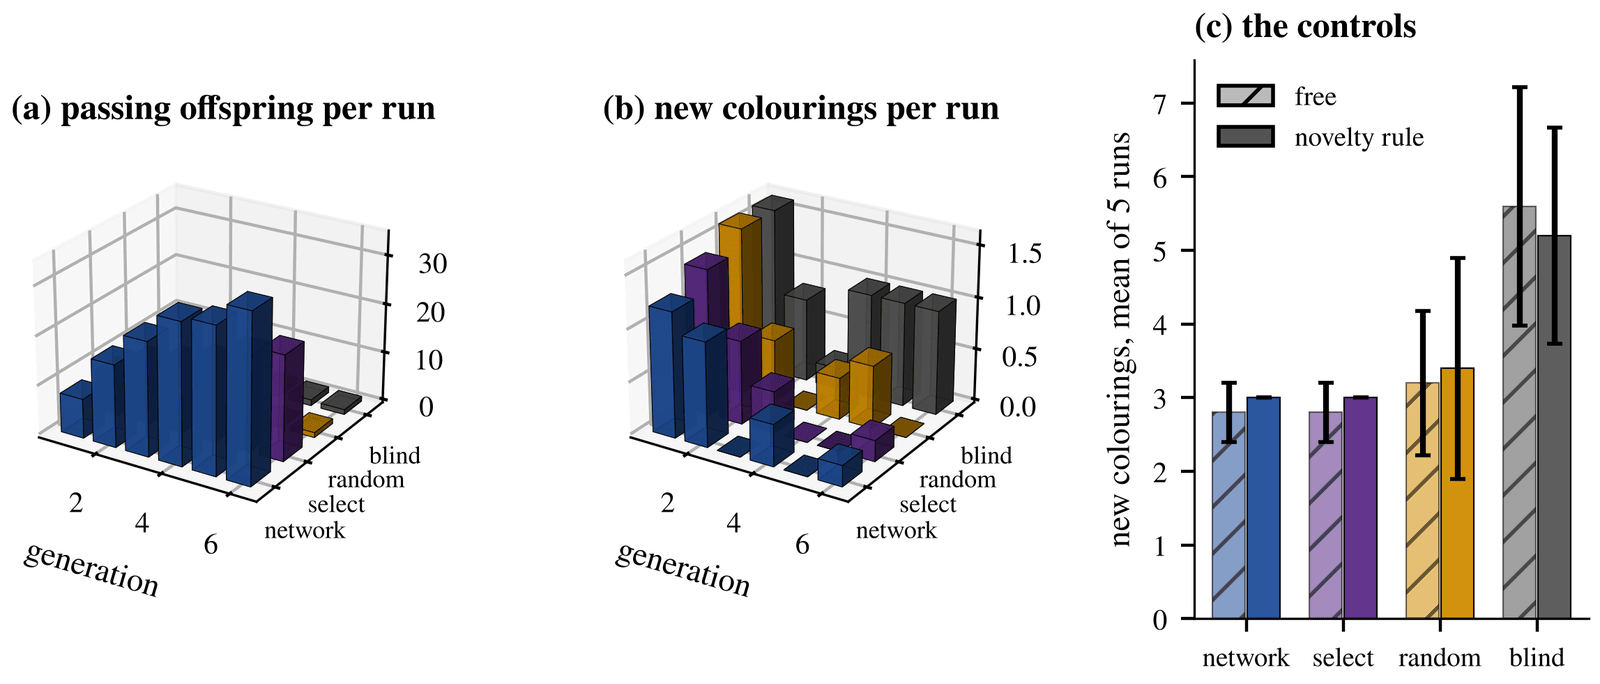
\includegraphics[width=0.98\textwidth]{figures/fig_crossing}
\Description{Curves of offspring passing the check and of new colourings per generation for the crossing network and its controls on Erdos problem 1183, and bars of new colourings per run.}
\caption{The crossing network against its controls on Erd\H{o}s problem 1183. (a) Offspring that pass the check, per generation, mean of five runs without the novelty rule. (b) Colourings not met before among them. (c) New colourings per run with and without the novelty rule, with one standard deviation. The network passes the most offspring and finds no more new colourings than the controls; the untyped arm finds the most.}
\label{fig:crossing}
\end{figure*}

\begin{table}[t]
\caption{The arms of the crossing network, five runs of $1200$ checks each. ``Pass'' is the share of offspring that pass the check; ``new'' is the number of new colourings per run (mean $\pm$ standard deviation) and ``optimal'' the number of them with $m(n)=f(n)$ for $n=6,\dots,9$. Ill-typed offspring are those of the blind arm that fail the typing.}
\label{tab:crossing}
\centering
\footnotesize
\setlength{\tabcolsep}{3.5pt}
\begin{tabular}{@{}lrrrr@{}}
\toprule
Arm & Pass & New & Optimal & Ill-typed \\
\midrule
\multicolumn{5}{@{}l}{\emph{free}}\\
network & $58.7\%$ & $2.8\pm0.4$ & $1.8$ & $0$ \\
select & $38.1\%$ & $2.8\pm0.4$ & $2.0$ & $0$ \\
random & $3.6\%$ & $3.2\pm1.0$ & $0.8$ & $0$ \\
blind & $2.7\%$ & $5.6\pm1.6$ & $1.6$ & $927$ \\
\multicolumn{5}{@{}l}{\emph{novelty rule}}\\
network & $1.3\%$ & $3.0\pm0.0$ & $2.0$ & $0$ \\
select & $1.4\%$ & $3.0\pm0.0$ & $2.0$ & $0$ \\
random & $1.4\%$ & $3.4\pm1.5$ & $1.0$ & $0$ \\
blind & $2.2\%$ & $5.2\pm1.5$ & $1.4$ & $1002$ \\
\bottomrule
\end{tabular}
\end{table}

\emph{The result} (Table~\ref{tab:crossing}). Without the novelty rule the network passes $58.7\%$ of its offspring against $3.6\%$ for random typed crossing, but almost all of them are colourings it has already found under another genome: it finds $2.8$ new colourings per run against $3.2$ for random crossing and $5.6$ for blind crossing. Under the novelty rule the pass rates fall to between $1.3\%$ and $2.2\%$ and the order of the new colourings is unchanged. The learned model therefore learns to repeat survivors, and it does not beat the random controls in the quantity that matters. Blind crossing does best because an untyped exchange occasionally grafts a family where a word was expected and so reaches combinations of the operations that typed crossing never proposes; the typing removes ill-formed genomes and, with them, part of the reachable set. None of the bred colourings improves a known value: the best, from the random arm, has $m(n)=7,7,8,8,9$ for $n=10,\dots,14$, which equals $f(n)$ at $n=11,13$ and exceeds it by one at $n=10,12,14$.

\emph{What did move the frontier} was a change of representation, not breeding. The optimal colourings found for $n=7,9,10$ by a counterexample-guided search over all colourings are level colourings, in which the colour of $S$ depends only on $|S|$; such a colouring is a word $c_{0}c_{1}\cdots c_{n}$, with colour classes $L_{0},L_{1}\subseteq\{0,\dots,n\}$. A \emph{weighted poset} is a finite poset $P$ with a map $w\colon P\to\{1,2,\dots\}$; $J(P)$ is its lattice of down-sets and $w(I)=\sum_{p\in I}w(p)$.

\begin{figure*}[t]
\centering
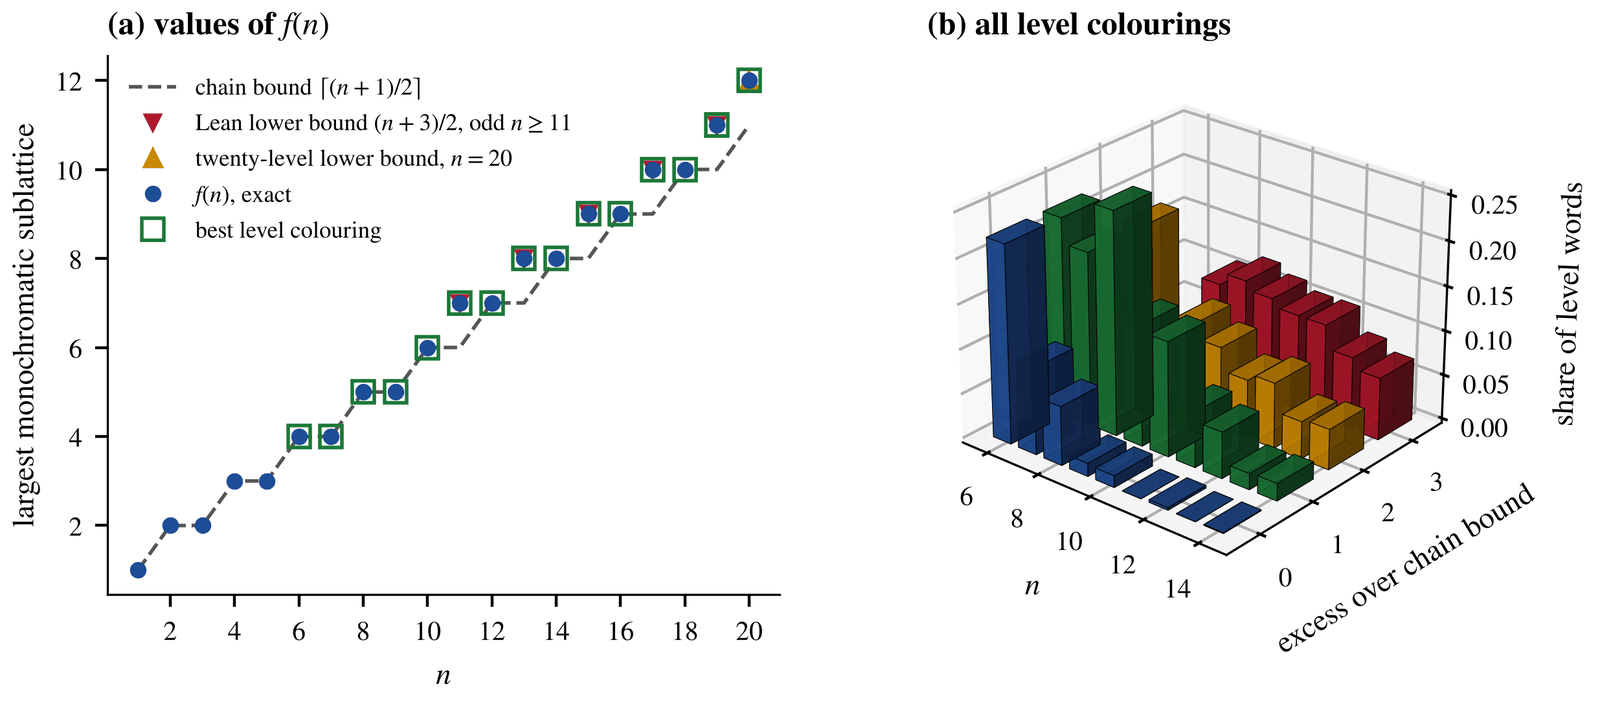
\includegraphics[width=0.98\textwidth]{figures/fig_sublattice}
\Description{The exact values of f(n) for n up to 20 against the chain bound and other bounds, and the distribution of the largest monochromatic sublattice over level colourings.}
\caption{Monochromatic sublattices of colourings of $2^{[n]}$. (a) The exact values of $f(n)$ for $n\le20$ (Theorem~\ref{thm:fvalues}), the chain bound $\lceil(n+1)/2\rceil$, the Lean lower bound $(n+3)/2$ for odd $n\ge11$ \cite{ORf1183}, the twenty-level lower bound $12$ at $n=20$, and the best level colouring, which attains $f(n)$ for every $n\le20$. (b) The distribution of the largest monochromatic sublattice over all level colourings for $6\le n\le14$, by its excess over the chain bound; the share of words that attain the bound falls quickly with $n$, and from $n=11$ on no odd word does.}
\label{fig:sublattice}
\end{figure*}

\begin{lemma}\label{lem:levelposet}
A level colouring has a monochromatic sublattice of colour class $L$ with $N$ members if and only if there are a weighted poset $(P,w)$ and an integer $t\ge0$ with $t+w(P)\le n$, $|J(P)|=N$ and $t+w(I)\in L$ for every $I\in J(P)$.
\end{lemma}

\begin{proof}
Let $D$ be a sublattice of $2^{[n]}$ with $N$ members whose sizes lie in $L$. It is a finite distributive lattice, so by Birkhoff's theorem it is isomorphic to $J(P)$ for the poset $P$ of its join-irreducible members, by the map that sends $A\in D$ to the set of join-irreducibles below it. The function $A\mapsto|A|$ is strictly increasing on $D$ and modular, since $|A\cup B|+|A\cap B|=|A|+|B|$. Write $p_{*}$ for the unique lower cover of a join-irreducible $p$ and $w(p)=|p|-|p_{*}|\ge1$. If $I$ is a down-set and $p$ a minimal element of $P\setminus I$, then $I\cup\{p\}$ is the join of $I$ and the principal down-set of $p$, and their meet is that principal down-set without $p$, which corresponds to $p_{*}$, so modularity gives $|I\cup\{p\}|=|I|+w(p)$; induction along a maximal chain of down-sets gives $|A|=t+w(I)$ with $t=|\min D|$, and $t+w(P)=|\max D|\le n$. Conversely, given $(P,w,t)$, choose disjoint sets $T$ and $B_{p}$ $(p\in P)$ in $[n]$ with $|T|=t$ and $|B_{p}|=w(p)$; the map $I\mapsto T\cup\bigcup_{p\in I}B_{p}$ is injective, carries unions and intersections of down-sets to unions and intersections of sets, and gives $I$ the size $t+w(I)\in L$.
\end{proof}

The lemma replaces the search over sublattices of $2^{[n]}$ by a search over weighted posets, which is small: the elements of $P$ are added in the order of the weights of their principal down-sets, each new element is placed above a down-set already built and creates the down-sets $I\cup\{p\}$ for every $I$ above that one, and a branch stops as soon as a new size leaves $L$. On $120$ random level colourings with $3\le n\le9$ the poset search and the general search agree on the largest monochromatic sublattice in every case, and on $30$ at $n=10$ they agree on every value below the cap of the poset search. A grid version, for colourings that depend on the sizes of $S$ in the blocks of a fixed partition of $[n]$, holds with weights in $\NN^{k}\setminus\{0\}$ by the same proof.

\begin{theorem}\label{thm:fvalues}
For $1\le n\le 19$,
\[
f(n)=\begin{cases}\lceil (n+1)/2\rceil & \text{if } n\le 10 \text{ or } n \text{ is even},\\[2pt] (n+3)/2 & \text{if } n\ge 11 \text{ is odd},\end{cases}
\]
and $f(20)=12$. For $11\le n\le20$ the value is attained by the level colouring of the word in the table below.
\begin{center}\small
\begin{tabular}{@{}rl@{\qquad}rl@{}}
$n$ & word $c_{0}\cdots c_{n}$ & $n$ & word $c_{0}\cdots c_{n}$\\
\midrule
$11$ & \texttt{110111001000} & $16$ & \texttt{10011001011100100}\\
$12$ & \texttt{1010011100100} & $17$ & \texttt{110100111001101000}\\
$13$ & \texttt{10111001101000} & $18$ & \texttt{0011001011100110100}\\
$14$ & \texttt{011010011100100} & $19$ & \texttt{00110010111000101101}\\
$15$ & \texttt{1100111010011000} & $20$ & \texttt{000101100111001011100}
\end{tabular}
\end{center}
\end{theorem}

\begin{proof}
The lower bounds are the chain bound and, for odd $n\ge11$, the theorem that every colouring then has a monochromatic sublattice with $(n+3)/2$ members, proved in Lean~4 by the OpenRefute project \cite{ORf1183}. For $n\le10$ the upper bound is attained by explicit colourings with no monochromatic sublattice of $\lceil(n+1)/2\rceil+1$ members, each checked by an exact search and by a satisfiability query that shares no code with it. For $11\le n\le19$ the words of the table have, by Lemma~\ref{lem:levelposet} and the exhaustive poset search, no monochromatic sublattice larger than the stated value; for $n=11$ this is confirmed by the exact search over all sublattices and by a satisfiability query. For $n=20$ the poset search finds $59$ level colourings of $2^{[20]}$, up to reversal and exchange of the colours, with no monochromatic sublattice of $13$ members, and the lower bound $f(20)\ge12$ is the twenty-level window of the footnote, which at $n=20$ gives a red and a blue sublattice with $23$ members together.
\end{proof}

The theorem answers the second part of the question of the footnote in the negative from $n=11$ on, as OpenRefute already did, and leaves the first open. Among level colourings (Fig.~\ref{fig:sublattice}) the chain bound is attained for every even $n\le18$ and exceeded by one for every odd $n$ from $11$ to $19$; up to reversal and exchange of the colours there are $9,7,6,8,3,2$ optimal words for $n=8,10,12,14,16,18$, and none for $n=20$, where the best level colouring has $12$ members against the chain bound $11$, and $12$ is $f(20)$. No optimal word for $n=8$ extends, two letters at a time on the right, through optimal words to $n=18$. The lemma shows the obstruction: three sizes of one colour in arithmetic progression already give a sublattice with one member more than the sizes, and a progression of length $d+1$ gives $2^{d}$ members, so a good word must avoid long monochromatic progressions in each colour class while the number of its colour changes grows with $n$. At $n=20$ no colouring at all attains the chain bound.

\emph{What the experiment shows.} The chain reaction was asked to produce new constructions faster than random crossing, and it did not; its survival model learned to propose what had already survived. The one advance on the problem came from a proof, Lemma~\ref{lem:levelposet}, that changed what could be checked: it turned the general search, which reaches $n=11$, into a search over weighted posets, which reaches $n=20$. In the terms of Theorem~\ref{thm:I}, the network sharpened the profile of a proposer whose support did not contain the needed idea; the lemma enlarged the support.

\subsection{Yang--Mills and Hodge: crossing on the open steps}\label{ssec:headline}

The crossing network of the package (Section~\ref{ssec:crossing} describes it on a calibration problem) is aimed here at the open leaves of the two trees. Every construction of its library is a typed node: it gives an output of one type and needs inputs of others. The Yang--Mills library holds the single-link law of $\mathrm{SU}(2)$, which is a von Mises--Fisher law on $S^{3}$; the sharp quarter inequality $W_{1}(\nu_{b},\nu_{b'})\le\frac14|b-b'|$ of \cite{BB26d}; Dobrushin's uniqueness criterion \cite{Dob68}; three dependency graphs of the links (no gauge fixing, temporal gauge, and the maximal-tree gauge of Creutz \cite{Cre77} with one fixed link in every plaquette); reflection positivity and the transfer matrix \cite{OSei78}; the gauge Dobrushin--Shlosman criterion and the Bakry--\'Emery bound of \cite{SZZ23}; the Polchinski flow and the multiscale log-Sobolev inequality \cite{BB21}; Ba{\l}aban's renormalisation group \cite{Bal87}; and a finite subgroup of $\mathrm{SU}(2)$. The Hodge library holds Markman's theorem on Weil classes of abelian fourfolds \cite{Mar25w}, the reduction of Moonen and Zarhin in dimension at most five \cite{MZ98}, Schoen's products \cite{Sch98p}, Shioda's structure of Fermat varieties \cite{Shi79}, the Hodge characters of the Fermat fourfold of degree $110$ left by the census of \cite{BB26c}, Buskin's theorem on Hodge isometries of K3 surfaces \cite{Bus19}, and an unrefereed claim of the Hodge conjecture for CM abelian varieties \cite{OAI26b}. Two nodes cross when the output of one is an input of the other. An offspring that needs nothing more is closed and goes to its check, a computation that accepts, rejects with the measurement that stopped it, or stops when no checkable form exists. Checked offspring join the pool and seed the next generation.

\begin{figure*}[t]
\centering
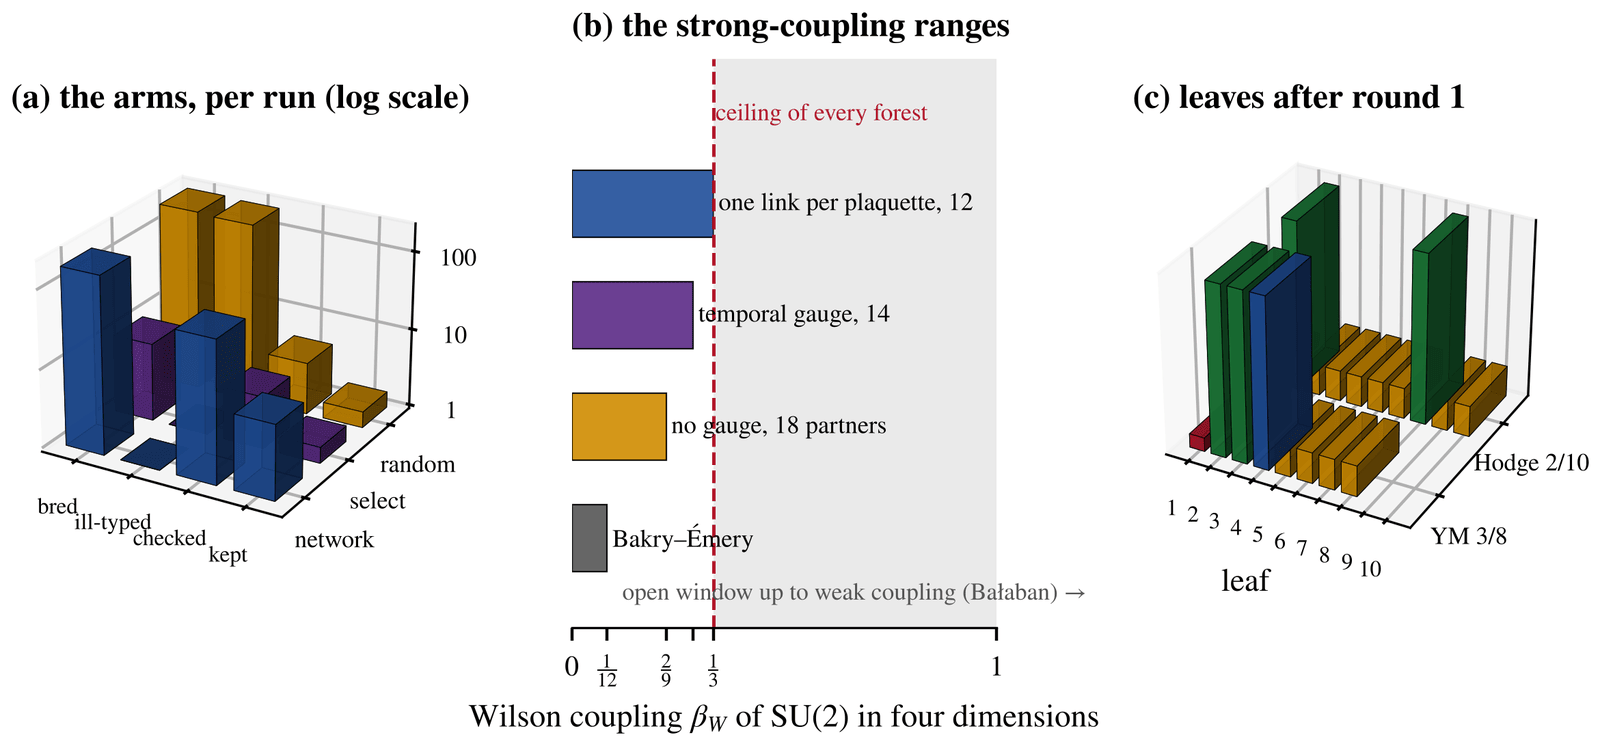
\includegraphics[width=0.98\textwidth]{figures/fig_headline}
\caption{The first headline round. (a) Offspring bred, ill-typed, checked and kept per run of each arm, on a logarithmic scale. The network enumerates the typed crosses; select draws pairs at random and keeps those whose types fit; random crosses whatever the types. (b) The ranges of four-dimensional $\mathrm{SU}(2)$ on which a lattice mass gap is proved: Bakry--\'Emery \cite{SZZ23}, single-link Dobrushin without gauge fixing \cite{BB26d}, and after the temporal and the one-per-plaquette gauge fixings (Theorem~\ref{thm:onethird}). The dashed line is the ceiling of every forest gauge fixing (Proposition~\ref{prop:forestceiling}); beyond it the window up to weak coupling is open. (c) The leaves of the two trees after the round, in the order of Table~\ref{tab:closure}: proved (green, the new step in blue), open (amber) and blocked (red).}
\label{fig:headline}
\end{figure*}

\emph{The first round.} Over five seeds of five generations of $40$ crosses, the network bred $180$ offspring per run, checked $64$ and accepted $8$; select bred $8.8$, checked $3.6$ and accepted $0.6$; random bred $200$, of which $191.2$ were ill-typed, and accepted $0.6$ (Fig.~\ref{fig:headline}a). Every run of the network reached the composite of Dobrushin's criterion, the sharp quarter, the von Mises--Fisher law and the maximal-tree gauge, whose check counts $12$ active partners for every active link and accepts the range $\beta_{W}<\frac13$; no run of the controls reached it. The network enumerates every typed pair, so its runs do not depend on the seed. The composite was first proposed by the language-model proposer of the package, which suggested fixing a gauge to cut the number of partners; a satisfiability search found the pattern of Lemma~\ref{lem:forest}, Lean~4 checked its finite part, and the cross was then entered in the library, from which the network rederives it. The network therefore reproduces this step; it did not originate it.

\emph{The step.} We use the normalisation of \cite{SZZ23,BB26d}: the Wilson measure of $\mathrm{SU}(2)$ on a finite set of links has density $\exp(2\beta\sum_{p}\mathrm{Re}\,\mathrm{Tr}\,U_{p})$ with respect to Haar measure, where $U_{p}$ is the ordered product around the plaquette $p$, and $\beta_{W}=4\beta$ is the coupling of the physics literature. A link of $\mathbb{Z}^{4}$ is written $(x,\mu)$ for the pair $\{x,x+e_{\mu}\}$; the plaquette at $x$ in the plane $\mu<\nu$ consists of the links $(x,\mu)$, $(x+e_{\mu},\nu)$, $(x+e_{\nu},\mu)$, $(x,\nu)$.

\begin{lemma}\label{lem:forest}
Let $\sigma\colon(\mathbb{Z}/2)^{4}\to\{0,1,2,3\}$ take the values $0,0,2,3,3,1,2,1,1,2,1,3,3,2,0,0$ at $x_{0}+2x_{1}+4x_{2}+8x_{3}=0,1,\dots,15$, and let $F$ be the set of links $(x,\sigma(x\bmod2))$, $x\in\mathbb{Z}^{4}$. Then
\begin{enumerate}[label=\textup{(\roman*)},leftmargin=*,itemsep=0pt]
\item every plaquette of $\mathbb{Z}^{4}$ contains exactly one link of $F$;
\item $F$ is a forest, and so is $F\cap E(\Lambda)$ for every set $\Lambda$ of sites, $E(\Lambda)$ being the links with both ends in $\Lambda$;
\item every link $e\notin F$ shares a plaquette with exactly $12$ links not in $F$, two in each of its six plaquettes.
\end{enumerate}
\end{lemma}

\begin{proof}
(i) The plaquette at $x$ in the plane $\mu<\nu$ contains $\#\{\sigma(x)\in\{\mu,\nu\}\}+[\sigma(x+e_{\mu})=\nu]+[\sigma(x+e_{\nu})=\mu]$ links of $F$, a number that depends only on $x\bmod2$ and the plane; inspection of the $16\times6=96$ cases of the table gives $1$ in each.\footnote{The inspection is a finite check. The eBLLM package carries it out in Lean~4, in the theorem \lean{one\_fixed\_per\_plaquette} of its file \lean{EBLLM/GaugeFix.lean}, proved by \lean{decide}, and repeated independently on a box of side six by \lean{verify\_gauge.py}. The table was found by a satisfiability search over the $4^{16}$ functions $\sigma$; it has eight solutions of period two, and none of period three.} (ii) Every site $x$ has exactly one link of $F$ leaving it in the positive direction, the link to $x+e_{\sigma(x)}$, and that link raises $h(x)=x_{0}+x_{1}+x_{2}+x_{3}$ by one. In a cycle of $k$ links of $F$ on $k$ sites, each link is the positive link of one of its ends and each site has at most one positive link, so each site of the cycle is the lower end of exactly one of its links and the cycle is directed; then $h$ increases strictly around it, which is impossible. A subgraph of a forest is a forest. (iii) A link lies in six plaquettes; by (i) each of them has exactly one link of $F$, which is not $e$, so it has two active links besides $e$. Two distinct plaquettes meet in at most one link, so the $12$ partners are distinct.
\end{proof}

On a periodic box $(\mathbb{Z}/L\mathbb{Z})^{4}$ the set $F$ contains cycles, since $h$ is not defined modulo $L$, and the argument below never uses a periodic box. Let $\gamma^{F}$ be the specification on the links of $\mathbb{Z}^{4}$ not in $F$ with a priori Haar measure and formal density $\exp(2\beta\sum_{p}\mathrm{Re}\,\mathrm{Tr}\,U^{F}_{p})$, where $U^{F}_{p}$ is the plaquette product with the links of $F$ replaced by $1$; for a box $\Lambda$ let $\mu^{F}_{\Lambda}$ be the finite-volume measure on the active links of $\Lambda$ with the plaquettes of $\Lambda$ only, and $W_{\Lambda}$ the Wilson measure on $E(\Lambda)$ with free boundary.

\begin{theorem}[Gauge-fixed strong coupling]\label{thm:onethird}
For four-dimensional $\mathrm{SU}(2)$ with $0\le\beta_{W}<\frac13$:
\begin{enumerate}[label=\textup{(\roman*)},leftmargin=*,itemsep=0pt]
\item $\gamma^{F}$ has exactly one Gibbs measure $\mu_{F}$, and its truncated correlations of Lipschitz local functions decay exponentially with every rate $\lambda<-\log(3\beta_{W})$ in the distance of their supports;
\item for every gauge-invariant local function $O$ the limit $\omega(O)=\lim_{\Lambda}W_{\Lambda}(O)$ exists along every sequence of boxes that exhausts $\mathbb{Z}^{4}$, and $\omega(O)=\mu_{F}(O^{F})$, where $O^{F}$ is $O$ with the links of $F$ set to $1$;
\item $\omega$ is invariant under translations and the hypercubic group and reflection positive, and its transfer matrix has a spectral gap $m\ge-\log(3\beta_{W})$.
\end{enumerate}
\end{theorem}

\begin{proof}
(i) The conditional law of an active link $e$ under $\gamma^{F}$ is the von Mises--Fisher law $\nu_{b}$ with $b=4\beta$ times the sum of the six staples of $e$, each staple being the product of the other links of a plaquette through $e$, with the links of $F$ equal to $1$. Moving an active link $e'$ moves at most one staple of $e$, since two links share at most one plaquette, and moves it by an isometric image of the displacement, since multiplication by unit quaternions is an isometry of $\RR^{4}$. By the sharp quarter inequality \cite[Theorem~A]{BB26d} the Dobrushin coefficient in the chordal metric of $S^{3}$ satisfies $C_{ee'}\le4\beta\cdot\frac14=\beta$, and $C_{ee'}=0$ unless $e'$ is one of the $12$ partners of Lemma~\ref{lem:forest}(iii). Every row and column of $C$ therefore sums to at most $\alpha=12\beta=3\beta_{W}<1$, and the Kantorovich--Dobrushin comparison lemma of \cite[Appendix]{BB26d} gives uniqueness and decay at every rate $\lambda<-\log\alpha$, exactly as in the proof of \cite[Theorem~E]{BB26d}.

(ii) Fix a box $\Lambda$. By Lemma~\ref{lem:forest}(ii) the set $F_{\Lambda}=F\cap E(\Lambda)$ is a finite forest. Root each of its trees and, given the values $U_{F}$ on $F_{\Lambda}$, define $g\colon\Lambda\to\mathrm{SU}(2)$ by $g=1$ at the roots and, along each tree, $g_{y}=g_{x}U_{xy}$ for every link $(x,y)$ of the tree; this is consistent because the tree has no cycle, and it makes $g_{x}U_{xy}g_{y}^{-1}=1$ on $F_{\Lambda}$. For fixed $U_{F}$ the map $U_{e}\mapsto g_{x}U_{e}g_{y}^{-1}$ on the active links is a product of left and right translations and preserves Haar measure, and the Wilson action is gauge invariant. Hence under $W_{\Lambda}$ the gauge-transformed active links are independent of $U_{F}$ and have law $\mu^{F}_{\Lambda}$, and $W_{\Lambda}(O)=\mu^{F}_{\Lambda}(O^{F})$ for gauge-invariant $O$. No holonomy is left over, because $F_{\Lambda}$ has no cycle. Now let $\Lambda\subset\Lambda'$ be boxes and compare $\mu^{F}_{\Lambda'}$ with $\mu^{F}_{\Lambda}\otimes\mathrm{Haar}$ on the active links of $\Lambda'$. Both are invariant under the single-link resampling of $\mu^{F}_{\Lambda'}$ at every active link all of whose plaquettes lie in $\Lambda$; the remaining links form a set $S$ within distance one of the complement of $\Lambda$. The comparison lemma of \cite[Appendix]{BB26d}, with $\theta=\alpha e^{\lambda}<1$, couples the two measures so that the expected distance on the support $T$ of $O^{F}$ is at most $\frac{2\theta}{1-\theta}\sum_{z\in S}e^{-\lambda\,\mathrm{dist}(z,T)}\le c_{T}\,R^{3}e^{-\lambda R}$, with $R=\mathrm{dist}(T,\mathbb{Z}^{4}\setminus\Lambda)$ and $c_{T}$ independent of $\Lambda'$. As $O^{F}$ is Lipschitz, $|W_{\Lambda'}(O)-W_{\Lambda}(O)|\le c_{O}R^{3}e^{-\lambda R}$. Any two boxes that contain the support at distance $R$ lie in a common larger box, so $W_{\Lambda}(O)$ converges along every exhausting sequence to one limit $\omega(O)$. The same coupling with $\mu_{F}$ in place of $\mu^{F}_{\Lambda'}$, which is invariant under all single-link resamplings of $\gamma^{F}$, gives $\omega(O)=\mu_{F}(O^{F})$.

(iii) For a translation or a symmetry $\tau$ of the lattice, $W_{\Lambda}(O\circ\tau)=W_{\tau\Lambda}(O)$ by the symmetry of the Wilson action, and the boxes $\tau\Lambda$ also exhaust $\mathbb{Z}^{4}$; by (ii) the limit is $\omega(O)$. Only the boxes move, not $F$. For a reflection $\vartheta$ in a lattice hyperplane through sites or bisecting links, the free-boundary measures $W_{\Lambda}$ on boxes symmetric under $\vartheta$ are reflection positive \cite{OSei78}, and by (ii) $\omega$ is their limit, so $\omega(\vartheta(\bar G)G)\ge0$ for every local $G$ supported on one side. Finally, for a gauge-invariant Lipschitz $G$ supported at times in $[0,s]$, part (i) applied to $\vartheta(\bar G)^{F}$ and $(\tau_{t}G)^{F}$, whose supports are at distance at least $t-s-1$, gives $0\le\omega(\vartheta(\bar G)\tau_{t}G)-|\omega(G)|^{2}\le C_{G}e^{-\lambda t}$. Such functions are dense in $L^{2}(\omega)$ on each bounded time interval, so \cite[Proposition~gapdecay]{BB26d} gives a gap at least $\lambda$ for every $\lambda<-\log(3\beta_{W})$.
\end{proof}

The theorem extends \cite[Theorem~F]{BB26d}, where the range is $\beta_{W}<\frac29$ and the state is the limit of periodic boxes, to $\beta_{W}<\frac13$, with the state the limit of free boxes. It has been checked here and not refereed. A search of the literature on strong-coupling expansions found no earlier statement of this range: \cite{OSei78} and the cluster expansions that followed give convergence at strong coupling without an explicit Dobrushin range, \cite{SZZ23} gives $\beta_{W}<\frac1{12}$, and the Lean project of strong-coupling lattice gauge theory cited in \cite{BB26d} has $\beta<1/(32n(d-1))$.\footnote{The search covered the arXiv listings in math-ph, hep-lat and math.PR, the citations of \cite{SZZ23}, the gauge-fixed formulations of Ba{\l}aban's renormalisation group, and the expository literature on maximal-tree gauges after \cite{Cre77}. The monograph of Seiler on gauge theories as statistical mechanics could not be read from the session, and its strong-coupling results are cluster expansions without an explicit range of the Dobrushin type.} The gain over \cite{BB26d} comes from the dependency graph and not from the metric: after a forest gauge fixing a plaquette has three active links instead of four, and each link loses six of its $18$ partners.

\begin{proposition}[The ceiling of forest gauge fixings]\label{prop:forestceiling}
Let $F'$ be any set of links of $\mathbb{Z}^{4}$ whose intersection with every box is a forest. Then the single-link Dobrushin coefficients of $\gamma^{F'}$, in the chordal or the geodesic metric of $S^{3}$, have $\sup_{e}\sum_{e'}C_{ee'}\ge12\beta$. Hence no single-link Dobrushin argument after a forest gauge fixing proves uniqueness for $\beta_{W}\ge\frac13$.
\end{proposition}

\begin{proof}
In a box of side $n$ there are $n^{4}$ sites, $4n^{4}-O(n^{3})$ links and $6n^{4}-O(n^{3})$ plaquettes, and a forest has at most $n^{4}-1$ links, so at least $3n^{4}-O(n^{3})$ links are active. Let $a_{p}$ be the number of active links of the plaquette $p$; then $\sum_{p}a_{p}=6\cdot\#\{\text{active links}\}-O(n^{3})$, since every link lies in six plaquettes, and the mean $\bar a$ of $a_{p}$ is at least $3-o(1)$. An active link $e$ has $\sum_{p\ni e}(a_{p}-1)$ active partners, so the sum of the partner counts over the active links is $\sum_{p}a_{p}(a_{p}-1)\ge\sum_{p}a_{p}\,(\bar a-1)$ by the Cauchy--Schwarz inequality, and the mean partner count is at least $6(\bar a-1)\ge12-o(1)$. Partner counts are integers, so some active link has at least $12$ partners. For each partner $e'$ of such a link, the staples of $e$ involve pairwise disjoint sets of other links and can be chosen with sum zero while the staple through $e'$ is arbitrary, and the proof of \cite[Proposition~ceiling]{BB26d} gives $C_{ee'}\ge\beta$.
\end{proof}

Passing to a weighted Dobrushin condition does not help either, since the spectral radius of a nonnegative matrix is at least its mean row sum over a box, up to the boundary.

\emph{The amplified round.} The second round adds to the library the crosses aimed at the assumption of each ceiling, the partners of the gauge-fixed specification, and the nodes obtained by transferring the pattern of the step that moved, \emph{remove redundant variables by a symmetry, then apply a local criterion}. It also passes every accepted offspring through a refuter before it counts, and adds the booster layer described below. Up to depth four the library breeds $21{,}515$ composites, of which $1{,}466$ are closed. Of these, $934$ stop without a checkable form, $433$ are rejected by their check, and $99$ are accepted. The refuter breaks $35$ of the accepted ones, $26$ because a stronger range is already known and $9$ because they reproduce an accepted range with no gain, and $64$ survive (Table~\ref{tab:amplify}).
\begin{itemize}[leftmargin=*,itemsep=1pt]
\item \emph{Plaquette variables} \cite{Bat82}. In these variables the Bianchi identity of each cube fixes every plaquette variable, up to parallel transport, by the other five plaquettes of the cube. The single-variable kernels are therefore point masses, so Dobrushin's coefficients equal one and the cross is rejected.
\item \emph{Blocks of active links.} A block coefficient needs the Kantorovich sensitivity of the joint law of a block at finite $\beta$, and the sharp quarter does not control it; the cross stops.
\item \emph{Path coupling.} The single-link Glauber dynamics contracts on exactly the Dobrushin range, so the cross gains nothing.
\item \emph{Bakry--\'Emery after the forest gauge fixing.} The Hessian of $\mathrm{Re}\,\mathrm{Tr}$ of a product of $k$ active links is at most $2k$ times the squared norm of the tangent vector. With three active links per plaquette instead of four, the curvature condition of \cite{SZZ23} improves from $\beta_{W}<\frac1{12}$ to $\beta_{W}<\frac19$, which the Dobrushin range dominates.
\item \emph{Dobrushin--Shlosman on a box of the gauge-fixed specification.} This needs the sensitivity of a box law to its boundary at order-one coupling, an integral over $\mathrm{SU}(2)^{3n^{4}}$; the estimate of \cite{BB26d} puts the box side near $90$, and the cross stops.
\item \emph{Pattern transfer to Fermat fourfolds.} Shioda's criterion is invariant under $\mu_{m}^{6}\rtimes S_{6}$ and under the Galois group. The leftover character $(1,16,26,31,36)$ at level $55$ has an orbit of $8$ members under the units of $\mathbb{Z}/55$, and none of them splits into zero-sum pairs and triples, so the quotient by the symmetries gives nothing new.
\item \emph{Pattern transfer to K3 squares.} For a K3 surface $S$ with real multiplication by $\mathbb{Q}(\sqrt d)$, the element $\sqrt d$ is a Hodge similitude $T(S)\to T(S)(d)$ and not an isometry, so Buskin's theorem does not apply to it. Composites through K3 surfaces $S'$ with $T(S')\cong T(S)(d)$ are similitudes too. Varesco reduces the algebraicity of Hodge similitudes to the Kuga--Satake Hodge conjecture \cite{Var23}, and he proves it on the first four-dimensional families. The transferred node therefore reproduces a known route, and it stops at the very general member of the larger families.
\end{itemize}

\begin{table}[t]
\caption{The amplified round on the two libraries, up to depth four. ``Survived'' counts accepted composites that the refuter could not break. The surviving Yang--Mills composites are $18$ forms each of the gap for $\beta_{W}<\frac29$, $<\frac27$ and $<\frac13$, and $3$ of uniqueness in each range; the Hodge survivor is (F2) in dimension at most five, which was known.}
\label{tab:amplify}
\centering
\footnotesize
\setlength{\tabcolsep}{4pt}
\begin{tabular}{@{}lrrrrr@{}}
\toprule
& Closed & Stopped & Rejected & Refuted & Survived \\
\midrule
Yang--Mills & $1{,}460$ & $932$ & $430$ & $35$ & $63$ \\
Hodge & $6$ & $2$ & $3$ & $0$ & $1$ \\
\midrule
Total & $1{,}466$ & $934$ & $433$ & $35$ & $64$ \\
\bottomrule
\end{tabular}
\end{table}

\subsection{Boosters}\label{ssec:boosters}

The booster layer of Section~\ref{sec:network} was tested on the Yang--Mills library at a budget at which no arm can enumerate every typed pair: $6$ crosses in each of $8$ generations, over $200$ seeds. Two forms were run, one synapse per pair of pool members and one per pair of library heads, so that a weight learned on one composite carries to every composite with the same heads; in a second experiment the boosted arm keeps its weights for four rounds (Fig.~\ref{fig:boosters}).

\begin{figure*}[t]
\centering
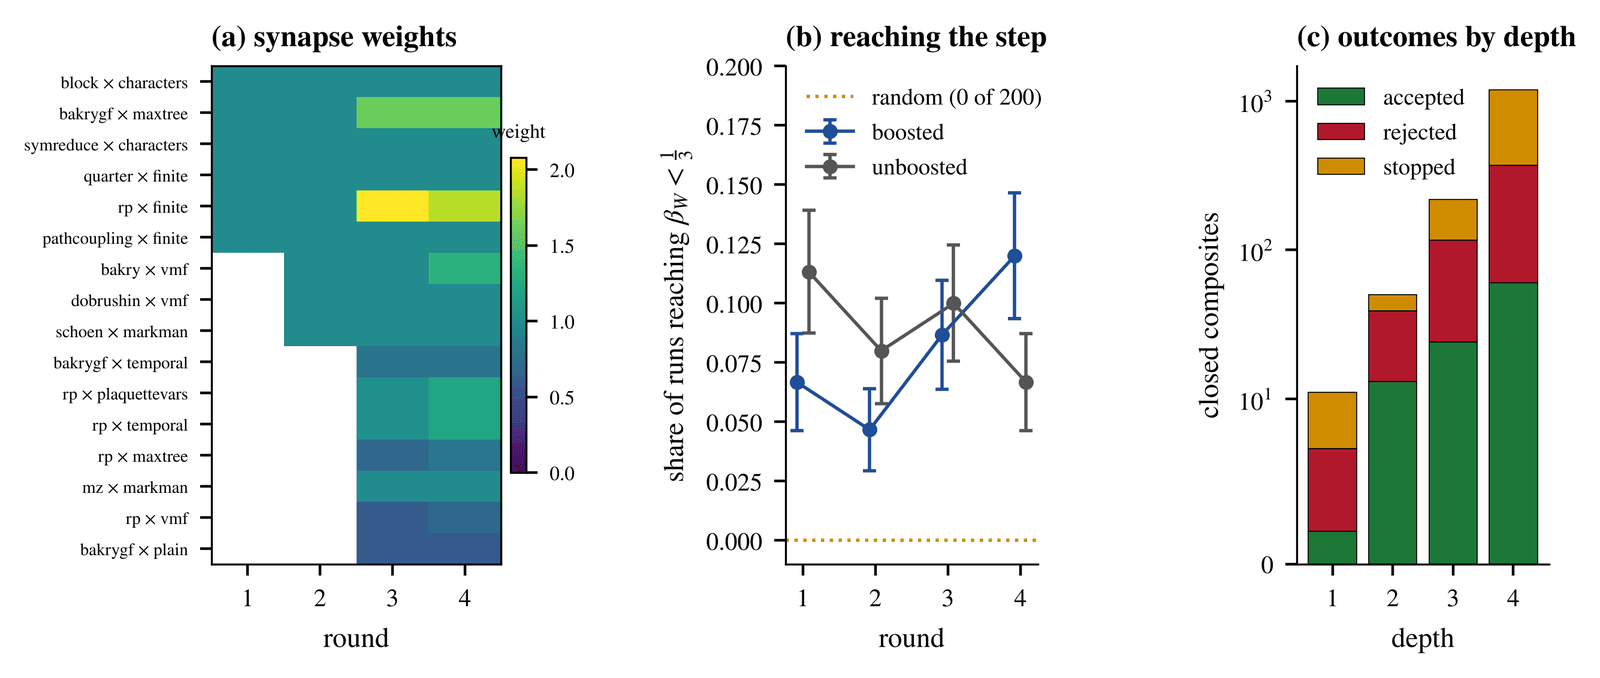
\includegraphics[width=0.98\textwidth]{figures/fig_boosters}
\caption{The booster layer. (a) The weights of the synapses of one boosted run over four rounds, one row per synapse; a blank cell is a synapse not yet created. (b) The share of $200$ runs that reach $\beta_{W}<\frac13$ within $48$ crosses, for the boosted arm that keeps its weights from round to round and for the unboosted network, with one standard error; random pairing never reaches it. (c) The outcomes of the $1{,}466$ closed composites of the amplified library, by depth.}
\label{fig:boosters}
\end{figure*}

\begin{table}[t]
\caption{Boosted, unboosted and random crossing at a budget of $48$ crosses, $200$ runs per arm. ``Reached $\frac13$'' counts runs whose survivors include $\beta_{W}<\frac13$, with the mean generation at which they reach it; survivors and refuted offspring are means per run.}
\label{tab:boosters}
\centering
\footnotesize
\setlength{\tabcolsep}{3.5pt}
\begin{tabular}{@{}llrrrr@{}}
\toprule
Synapse & Arm & Reached $\frac13$ & Generation & Survivors & Refuted \\
\midrule
pair & boosted & $14$ & $5.86$ & $0.61$ & $1.14$ \\
head & boosted & $12$ & $5.58$ & $0.62$ & $1.16$ \\
-- & unboosted & $21$ & $5.43$ & $0.68$ & $1.25$ \\
-- & random & $0$ & -- & $0.08$ & $0.05$ \\
\bottomrule
\end{tabular}
\end{table}

Boosters do not beat the unboosted network (Table~\ref{tab:boosters}). Within one round the boosted arms reach the step in $12$ and $14$ of $200$ runs against $21$ for the unboosted network; the difference is within two standard errors. Across four rounds the boosted share moves from $0.067$ to $0.12$ and the unboosted share from $0.113$ to $0.067$, again within two standard errors in every round. Both are far above random pairing, which wastes $45$ of its $48$ crosses on ill-typed pairs and never reaches the step. The reason is the one met in Section~\ref{ssec:crossing}: a booster strengthens synapses that have already fired, and the step that moved needed a synapse that had never fired, between Dobrushin's criterion and the maximal-tree gauge. The typing, not the learning, carries the advantage of the network.

\subsection{Gap numbers and the construction graph}\label{ssec:gapnumbers}

\emph{Gap numbers.} Each round reports two numbers. For Yang--Mills it is the largest coupling below which the lattice gap is proved, and its share of the interval up to $\beta_{W}\approx2.2$, where Monte Carlo simulations of four-dimensional $\mathrm{SU}(2)$ see the crossover from strong to weak coupling \cite{Cre80}; this is a physical marker and not the threshold of any proof, since Ba{\l}aban's control is not explicit in the coupling. The number moved from $\frac29$, or $10.1\%$, before the rounds to $\frac13$, or $15.2\%$, in the first round, and stayed there in the second. For Hodge it is, for each open family, the largest dimension of a family on whose general member the classes are known to be algebraic, against the dimension of the largest family of its kind (Table~\ref{tab:closure}). No Hodge number moved.

\begin{table*}[t]
\caption{The leaves of the two benchmark trees after the second round, with the result that settles a proved leaf, the check that stopped the last attempt on an open one, and, for the open families of the Hodge tree, the gap number: the largest dimension of a family on whose general member the classes are known to be algebraic, against the dimension of the largest family of its kind. Yang--Mills: $3$ of $8$ leaves proved ($37.5\%$); Hodge: $2$ of $10$ ($20\%$).}
\label{tab:closure}
\centering
\footnotesize
\setlength{\tabcolsep}{4pt}
\begin{tabular}{@{}rp{0.22\textwidth}p{0.08\textwidth}p{0.55\textwidth}p{0.07\textwidth}@{}}
\toprule
& Leaf & Status & Source, or what blocks & Gap \\
\midrule
\multicolumn{5}{@{}l}{\emph{Yang--Mills}}\\
\rr 1 & \rr a faithful Lean statement of the Clay problem & \rr blocked & \rr no formal statement of the Wightman axioms for a gauge theory exists to state it against & \rr -- \\
\rr 2 & \rr lattice gap at strong coupling & \rr proved & \rr $\beta_{W}<\frac29$ \cite{BB26d} & \rr -- \\
\rr 3 & \rr fine-scale control at weak coupling & \rr proved & \rr Ba{\l}aban's renormalisation group \cite{Bal87} & \rr -- \\
\rr 4 & \rr the window from below & \rr proved & \rr $\beta_{W}<\frac13$, Theorem~\ref{thm:onethird}; the ceiling of the method, Proposition~\ref{prop:forestceiling} & \rr $15.2\%$ \\
\rr 5 & \rr a finite-box mixing certificate in the window & \rr open & \rr the box needs side about $90$; no computation over $\mathrm{SU}(2)^{4n^{4}}$ at that size exists & \rr -- \\
\rr 6 & \rr a lift of the two-dimensional gap through dimension & \rr open & \rr no family of theories interpolating in dimension with a uniform gap is known & \rr -- \\
\rr 7 & \rr a multiscale log-Sobolev inequality at order-one coupling & \rr open & \rr the method of \cite{BB21} needs a Polchinski flow with uniformly convex effective potentials; for gauge fields none is known, and gauge invariance removes the Gaussian reference measure & \rr -- \\
\rr 8 & \rr the continuum limit with the Wightman axioms & \rr open & \rr needs a lattice gap uniform in the spacing, Hypothesis~R, which is the Clay problem on the lattice & \rr -- \\
\midrule
\multicolumn{5}{@{}l}{\emph{Hodge}}\\
\rr 1 & \rr a faithful Lean statement & \rr blocked & \rr Hodge classes and algebraic cycles of complex projective varieties are not yet formalised & \rr -- \\
\rr 2 & \rr (F2) in dimension at most five & \rr proved & \rr \cite{Mar25w,MZ98} & \rr -- \\
\rr 3 & \rr (F2) for CM abelian varieties & \rr open & \rr the only claim is unrefereed \cite{OAI26b}; the refuter rejects it & \rr -- \\
\rr 4 & \rr Weil classes on Weil eightfolds of nontrivial discriminant & \rr open & \rr no construction of the classes is known & \rr $0/16$ \\
\rr 5 & \rr a semiregular object on $E_{0}^{6}$ meeting the polarised criterion & \rr open & \rr every convolution tested in \cite{BB26c} has too large an $\mathrm{Ext}^{2}$ & \rr -- \\
\rr 6 & \rr Weil classes on Weil sixfolds & \rr open & \rr products of Weil fourfolds and Weil surfaces fill a family of dimension $5$ in the moduli of dimension $9$; a very general Weil sixfold is simple & \rr $5/9$ \\
\rr 7 & \rr (F3$'$) for $S\times S$, $S$ a K3 surface with real multiplication & \rr open & \rr $\sqrt d$ is a Hodge similitude; Varesco's reduction to the Kuga--Satake Hodge conjecture \cite{Var23} covers the first four-dimensional families, the largest family has dimension $8$ & \rr $4/8$ \\
\rr 8 & \rr Fermat fourfolds, degrees with split characters & \rr proved & \rr Shioda's zero-sum criterion \cite{Shi79} with the census of \cite{BB26c} & \rr -- \\
\rr 9 & \rr the Fermat fourfold of degree $110$ & \rr open & \rr the leftover character has a lattice point in its Fine interior, so no block family covers it, and its orbit under the symmetries has no split member & \rr one orbit \\
\rr 10 & \rr the Fermat fourfold of degree $220$ & \rr open & \rr the classes lifted from degree $110$ & \rr -- \\
\bottomrule
\end{tabular}
\end{table*}

\emph{What blocks.} On Yang--Mills the step that blocks is Hypothesis~R: a lattice gap uniform in the spacing, for which Ba{\l}aban's effective action at a fixed physical scale must land in a region where a convergent method applies. The strong-coupling side now reaches $\beta_{W}=\frac13$, the ceiling of single-link arguments after any forest gauge fixing, and going further needs multi-link blocks whose joint laws are controlled at finite coupling. On Hodge every open leaf is blocked by the absence of a construction of the classes: of Weil classes off the products of lower Weil varieties, of the classes of $\sqrt d$ on squares of K3 surfaces outside Varesco's families, and of the leftover class of the Fermat fourfold of degree $110$.

\emph{The construction graph.} The package records every node, every crossing with its parents, check and refuter verdict, the synapse weights of every run, and the map of the other workstreams that feed the library (Fig.~\ref{fig:graph}). Four workstreams feed it. The Yang--Mills archive \cite{BB26d} gives the sharp quarter, reflection positivity and the box criterion; the Hodge papers \cite{BB26c} give the split into (F2) and (F3$'$) and the open families; the census of Fermat varieties gives the characters left at $110$ and $220$; and the weighted-poset lemma of Section~\ref{ssec:crossing} gives the pattern of a change of representation, which the amplified round transfers to plaquette variables, blocks and the quotient of Fermat characters. The work on the lattice $D_{4}$ and the $24$-cell gives the pattern of a finite certificate, which the box nodes use. The Lehmer and Earth--Moon workstreams feed neither tree.

\begin{figure*}[t]
\centering
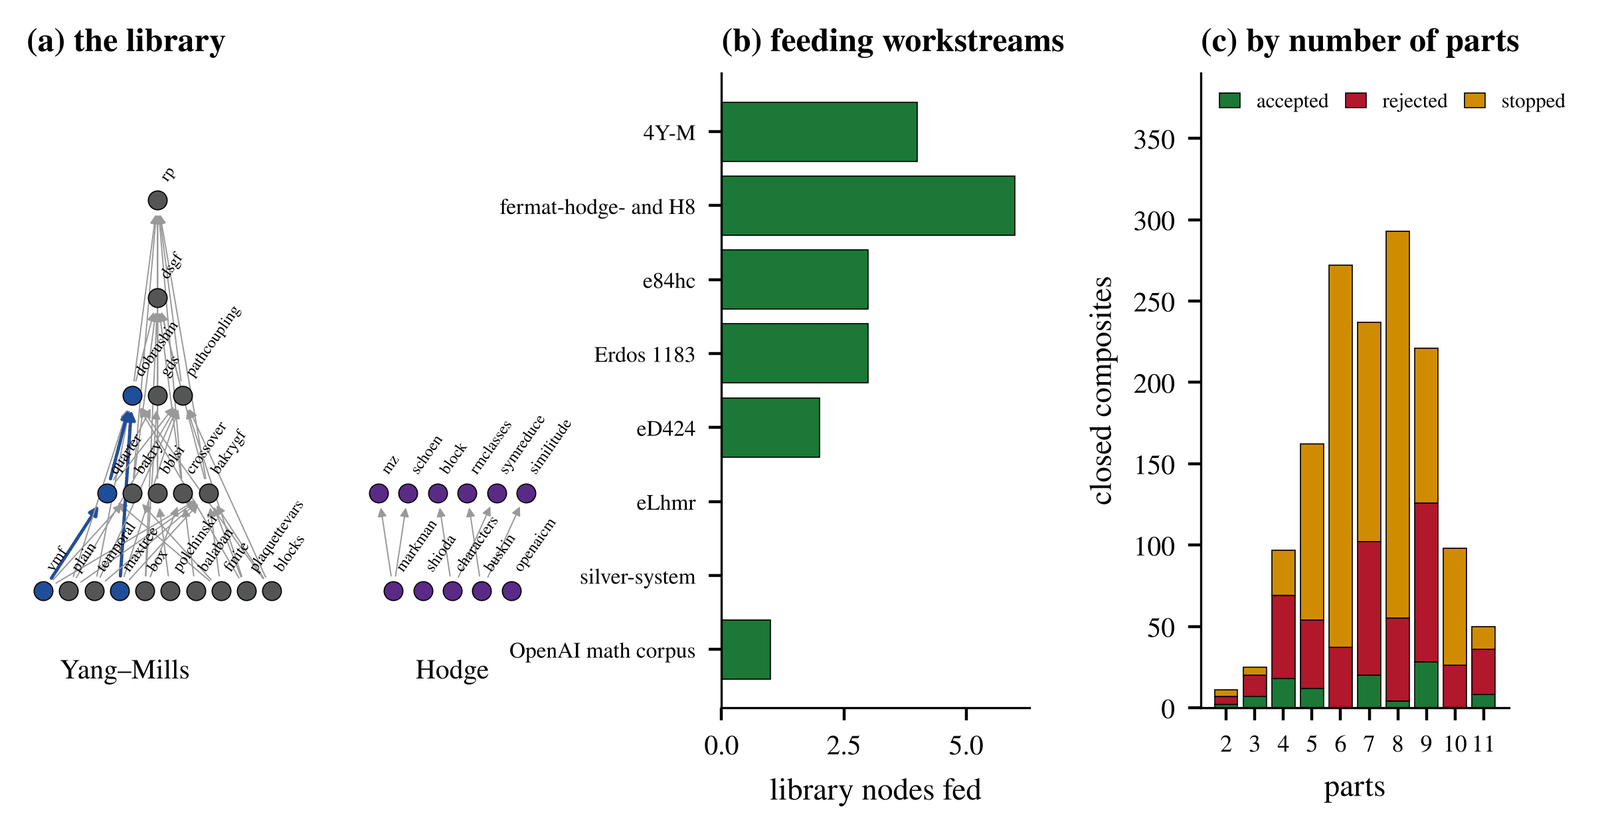
\includegraphics[width=0.98\textwidth]{figures/fig_graph}
\caption{The construction graph. (a) The library of the amplified round, with an arrow from $b$ to $a$ when $b$ can be fed into $a$, layered by the length of the longest chain of inputs; Yang--Mills nodes on the left, Hodge nodes on the right, and the four parents of the composite that proves $\beta_{W}<\frac13$ in blue. (b) The number of library nodes fed by each workstream. (c) Closed composites of the amplified library by number of parts and outcome.}
\label{fig:graph}
\end{figure*}

\subsection{Memory}\label{ssec:memory}

The memory study runs the whole package over the five libraries for $5$ rounds and $60$ seeds, with $8$ generations of $10$ crosses per round, in five arms: the full system (boosters, memory, retrieval, the committee of proposers); the full system without retrieval, which keeps the memory but does not let it steer; boosters alone; no boosters; and random pairing. Every arm without memory starts each round from the library and keeps only its synapse weights. The measured quantities are the distinct survivors after each round and the checks spent on them (Fig.~\ref{fig:memory}).

\begin{figure*}[t]
\centering
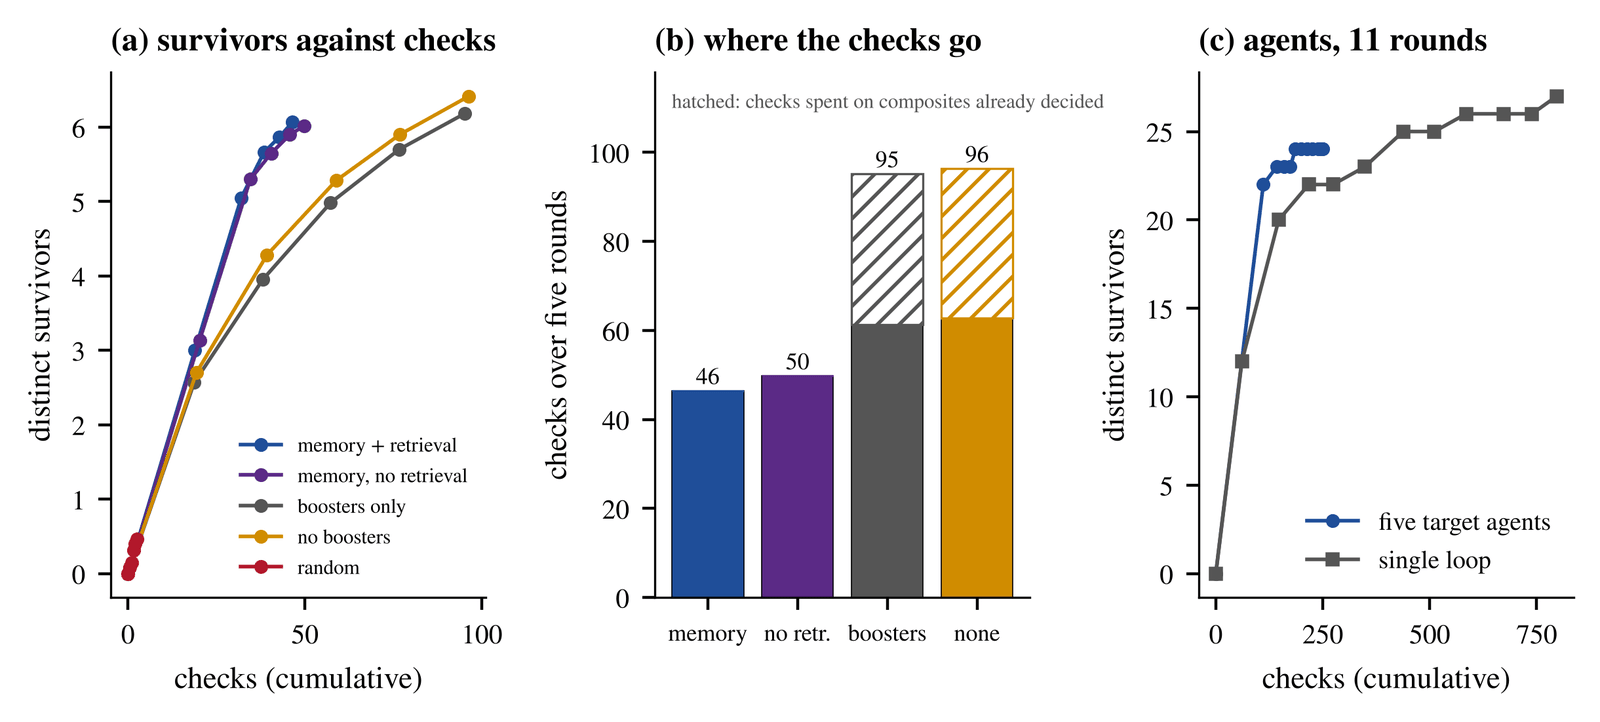
\includegraphics[width=0.98\textwidth]{figures/fig_memory}
\Description{Curves of distinct survivors against cumulative checks over five rounds, bars of checks with the part spent on already decided composites hatched, and five target agents against the single loop.}
\caption{Memory and agents. (a) Distinct survivors against cumulative checks over five rounds, mean of $60$ seeds; each marker is one round. (b) Checks over the five rounds; the hatched part is spent on composites that an earlier round of the same seed had already decided. (c) The five target agents against the single-loop control in the continuous loop, with the local model among the proposers; each marker is one round.}
\label{fig:memory}
\end{figure*}

\begin{table}[t]
\caption{The memory study: five rounds, $60$ seeds, means per seed. ``Repeated'' counts checks of composites decided in an earlier round.}
\label{tab:memory}
\centering
\footnotesize
\setlength{\tabcolsep}{3.5pt}
\begin{tabular}{@{}lrrrr@{}}
\toprule
Arm & Checks & Repeated & Survivors & Refuted \\
\midrule
full system & $46.4$ & $0.0$ & $6.07$ & $5.2$ \\
no retrieval & $49.8$ & $0.0$ & $6.02$ & $5.3$ \\
boosters only & $95.2$ & $33.9$ & $6.18$ & $10.6$ \\
no boosters & $96.3$ & $33.6$ & $6.42$ & $10.6$ \\
random & $2.5$ & $0.1$ & $0.47$ & $0.3$ \\
\bottomrule
\end{tabular}
\end{table}

Every arm except random pairing ends between $6.0$ and $6.4$ distinct survivors, because the five libraries hold that many checkable statements within reach of the crosses; all of them are known results. The arms differ in cost (Table~\ref{tab:memory}). With memory the system reaches the plateau with $46.4$ checks, against $95.2$ for boosters alone, and spends none on composites already decided; without memory a third of the checks after the first round are repeats. Retrieval steers the draw but changes little, $46.4$ checks against $49.8$: the saving comes from not checking a decided composite twice, which is the soundness bookkeeping of Section~\ref{sec:chains} applied across rounds. Memory therefore halves the cost of reaching what the libraries can reach, and it does not move the plateau.

\subsection{The channel and the agents}\label{ssec:agentsexp}

The channel study runs the five agents on one shared memory for $6$ rounds and $60$ seeds in three arms: the channel with the target weights, the target weights alone, and neither. The three arms spend $211.8$, $218.0$ and $216.8$ checks per seed over the six rounds, with standard errors below one check, and end with $24.05$, $24.15$ and $24.23$ distinct survivors. The channel saves three per cent of the checks, because a bundle that carries a failed cell halves the weight of its candidate, and it costs a tenth of a survivor for the same reason. In none of the $180$ runs does a survivor reach a target point. The channel delivers everything the engine holds, and what the engine holds are outputs of library constructions; no library holds the input that a target point needs (Section~\ref{ssec:whyhard}).

The continuous loop runs the five agents and, beside them, a single-loop control: one attack over all five libraries with boosters and no memory, $6$ generations of $40$ crosses per round. The agents use the channel, the target weights and the local model. After eleven rounds the agents hold $24$ distinct survivors for $250$ checks and the control $27$ for $797$ (Fig.~\ref{fig:memory}(c)). The agents reach $23$ survivors in the second round, for $142$ checks, and $24$ in the fifth; the control needs five rounds and $348$ checks to reach $23$ and passes the agents in the sixth round, still adding a known result every few rounds at about $70$ checks per round. No survivor of either reaches a target point. Agents are cheaper for the same reason as memory, since each agent skips what its slice of the store has decided, and they reach no further, since a target point needs an input that no library holds; the control's three extra survivors are known results that the agents' narrower libraries do not contain.

\subsection{The barrier and pattern matrix}\label{ssec:matrix}

The last experiment is done by hand and recorded in the package. For each blocking step, every pattern that broke a comparable barrier elsewhere is transferred, and the transferred statement, its needed input and the outcome are written as one cell: \emph{closes} when the pass line is crossed, \emph{partial} when a weaker statement follows or a new fact is computed, \emph{fails} when the needed input is false or unknown, with the reason. There are $38$ cells. None closes; $7$ are partial and $31$ fail. The partial cells are the forest gauge fixing and its ceiling, the box Dobrushin--Shlosman criterion as a finite check not yet run, size colourings and Theorem~\ref{thm:fvalues}, the forced arithmetic progressions in level colourings, the Kuga--Satake reduction of Varesco, the averaged Chowla theorem, and the grid search at $n=20$. The failures fall into three kinds: the input is known to be false (product colourings and m-sequence colourings for Erd\H{o}s problem 1183, plaquette variables, abelian duality for $\mathrm{SU}(2)$), the input is the open problem itself or another benchmark (motivated cycles, which are algebraic exactly when the standard conjecture holds; the inverse of $L$ as a Hodge class on $X\times X$), or the input needs a small parameter that is not small at the blocking step (Ba{\l}aban, Brydges--Yau, Kotecký--Preiss). The matrix is the content of the cells $\pi_{\mathrm{ch}}$ of \eqref{eq:channelprior} reads, so a pattern recorded as failing on a benchmark is drawn half as often there.

Two cells are new computations and one is a new negative result.

\begin{proposition}\label{prop:productrules}
Let $c_{1},c_{2}$ be level colourings of $2^{[a]}$ and $2^{[b]}$ attaining $f(a)$ and $f(b)$, and colour $S\subseteq[a+b]$ by $\phi(c_{1}(S\cap[a]),c_{2}(S\setminus[a]))$ for a Boolean function $\phi$ of two variables that depends on both. For $a=b=4$ the largest monochromatic sublattice has $16$ members when $\phi$ is exclusive or or its negation, $32$ for disjunction and $48$ for conjunction, against $f(4)+f(4)=6$.
\end{proposition}

The grid search of Lemma~\ref{lem:levelposet}, run with two blocks, computes these values. They show why subadditivity $f(a+b)\le f(a)+f(b)+C$ cannot come from such products: a monochromatic sublattice of the product projects to sublattices of the factors, but the colour of a product point is a function of both factors, so the projections need not be monochromatic, and the product lattice of two chains is a grid with $(a+1)(b+1)$ members.

At $n=20$ the grid colourings with two blocks of sizes $18$ and $2$, $57$ grid points, were searched by simulated annealing on the number of pairs (colour, base point) from which a monochromatic sublattice of $12$ members is reachable. Of $24$ restarts, $16$ end with exactly one such pair and none with zero; every colouring obtained from the best one by changing one or two grid points keeps a bad pair. Refining the best colouring to three blocks of sizes $(16,2,2)$ and $(17,1,2)$ and annealing again, four restarts, also ends at one bad pair. None of the runs reaches zero, and none can: by the twenty-level window cited in Theorem~\ref{thm:fvalues}, every colouring of $2^{[20]}$ has a monochromatic sublattice of $12$ members.

The colourings with the shortest monochromatic progressions known come from finite fields, and they were the natural candidates for an answer to Question~9.3. They fail.

\begin{proposition}\label{prop:mseq}
Let $\alpha$ be a primitive element of $\mathbb{F}_{2^{p}}$, $\beta\neq0$, $n\le2^{p}-2$, and colour $S\subseteq[n]$ by $\mathrm{Tr}(\beta\alpha^{|S|})$. \textup{(i)} If $p$ is prime, every monochromatic sublattice isomorphic to a Boolean lattice has at most $2^{p-1}$ members. \textup{(ii)} If $\alpha^{e}=1+\alpha^{d}$ and $\mathrm{Tr}(\beta\alpha^{t+jd})=0$ for $0\le j\le k$, with $t+k\max(d,e)\le n$, there is a monochromatic sublattice with $3^{k}$ members. If $\alpha$ is a root of the trinomial $x^{p}+x+1$ and $n=2^{p}-2$, a suitable $\beta$ allows $d=1$, $e=p$, $t=0$ and $k=p-2$, which gives $3^{p-2}=\frac19(n+2)^{\log_{2}3}$ members.
\end{proposition}

\begin{proof}
A Boolean sublattice of rank $k$ is $J(P)$ for an antichain $P=\{1,\dots,k\}$ with weights $w_{i}$ and base $t$, and its members have colours $\mathrm{Tr}(\beta x)$ for $x$ in $X=\{\alpha^{t}\prod_{i\in I}\alpha^{w_{i}}\}$, whose span is $\alpha^{t}\prod_{i}\mathrm{span}\{1,\alpha^{w_{i}}\}$; each factor is a plane, since $1\le w_{i}\le2^{p}-2$. For prime $p$ the field $\mathbb{F}_{2^{p}}$ has no subfield other than $\mathbb{F}_{2}$ and itself, so the theorem of Hou, Leung and Xiang \cite{HLX02} gives $\dim(UV)\ge\min(p,\dim U+\dim V-1)$ for nonzero subspaces $U,V$, and the span has dimension at least $\min(p,k+1)$. Colour $0$ puts it in a hyperplane, so $k\le p-2$. For colour $1$ the differences $\alpha^{t}(1+\alpha^{w_{j}})\prod_{i\in I}\alpha^{w_{i}}$, $I\not\ni j$, have trace $0$ and span a product of $k-1$ planes times one element, so $k\le p-1$. This is (i). For (ii) take $k$ disjoint chains, each with ranks $0$, $d$ and $e$. Their down-sets have ranks $t+ad+be$ with $a+b\le k$, and $\alpha^{t+ad+be}=\alpha^{t}(\alpha^{d})^{a}(1+\alpha^{d})^{b}$ lies in the span of $\alpha^{t},\alpha^{t+d},\dots,\alpha^{t+kd}$, so every member has trace $0$, and $t+k\max(d,e)\le n$ keeps all ranks in range. The sublattice has $3^{k}$ members. For the trinomial, $\alpha^{p}=1+\alpha$, and the condition asks for a run of $k+1$ zeros in the $m$-sequence $\mathrm{Tr}(\beta\alpha^{i})$; each period has a run of $p-1$ zeros, choosing $\beta$ moves it to $t=0$, and $(p-2)p\le2^{p}-2$.
\end{proof}

For the colourings defined by $x^{5}+x^{2}+1$, $x^{6}+x+1$ and $x^{7}+x+1$ at $n=2^{p}-2$, the largest sublattices of the form (ii) have $27$, $81$ and $243$ members, or $0.84$, $1.27$ and $1.90$ times $n+2$, with $(d,e)=(2,5)$, $(1,6)$ and $(1,7)$. The linearity that keeps the progressions of both classes at length $p-1$ turns every progression whose difference has a small partner $e$ into a triangle of ranks, so an answer to Question~9.3 by level colourings needs classes that avoid both.

